\chapter{Related work}
\label{cha:Figures}

A main approach for non-rigid registration is proposed by Anguelov \cite{Anguelov04} applying the correlated correspondence algorithm \cite{CorrelatedCorrespondance}. 
%%
\subsection{Correlated Correspondence}
The algorithm takes a \textit{template} Mesh $D_0$ and other Meshes $D_1,\ldots,D_n$ in different configurations as input. The algorithm then performs a probabilistic framework and Expectation-Maximization (EM) to iterate between finding a decomposition of the \textit{template} into rigid parts and detecting them in the other meshes. Furthermore, a random clustering is applied to facilitate the detection of associated rigid parts.
%%
\begin{figure}
	\centering
	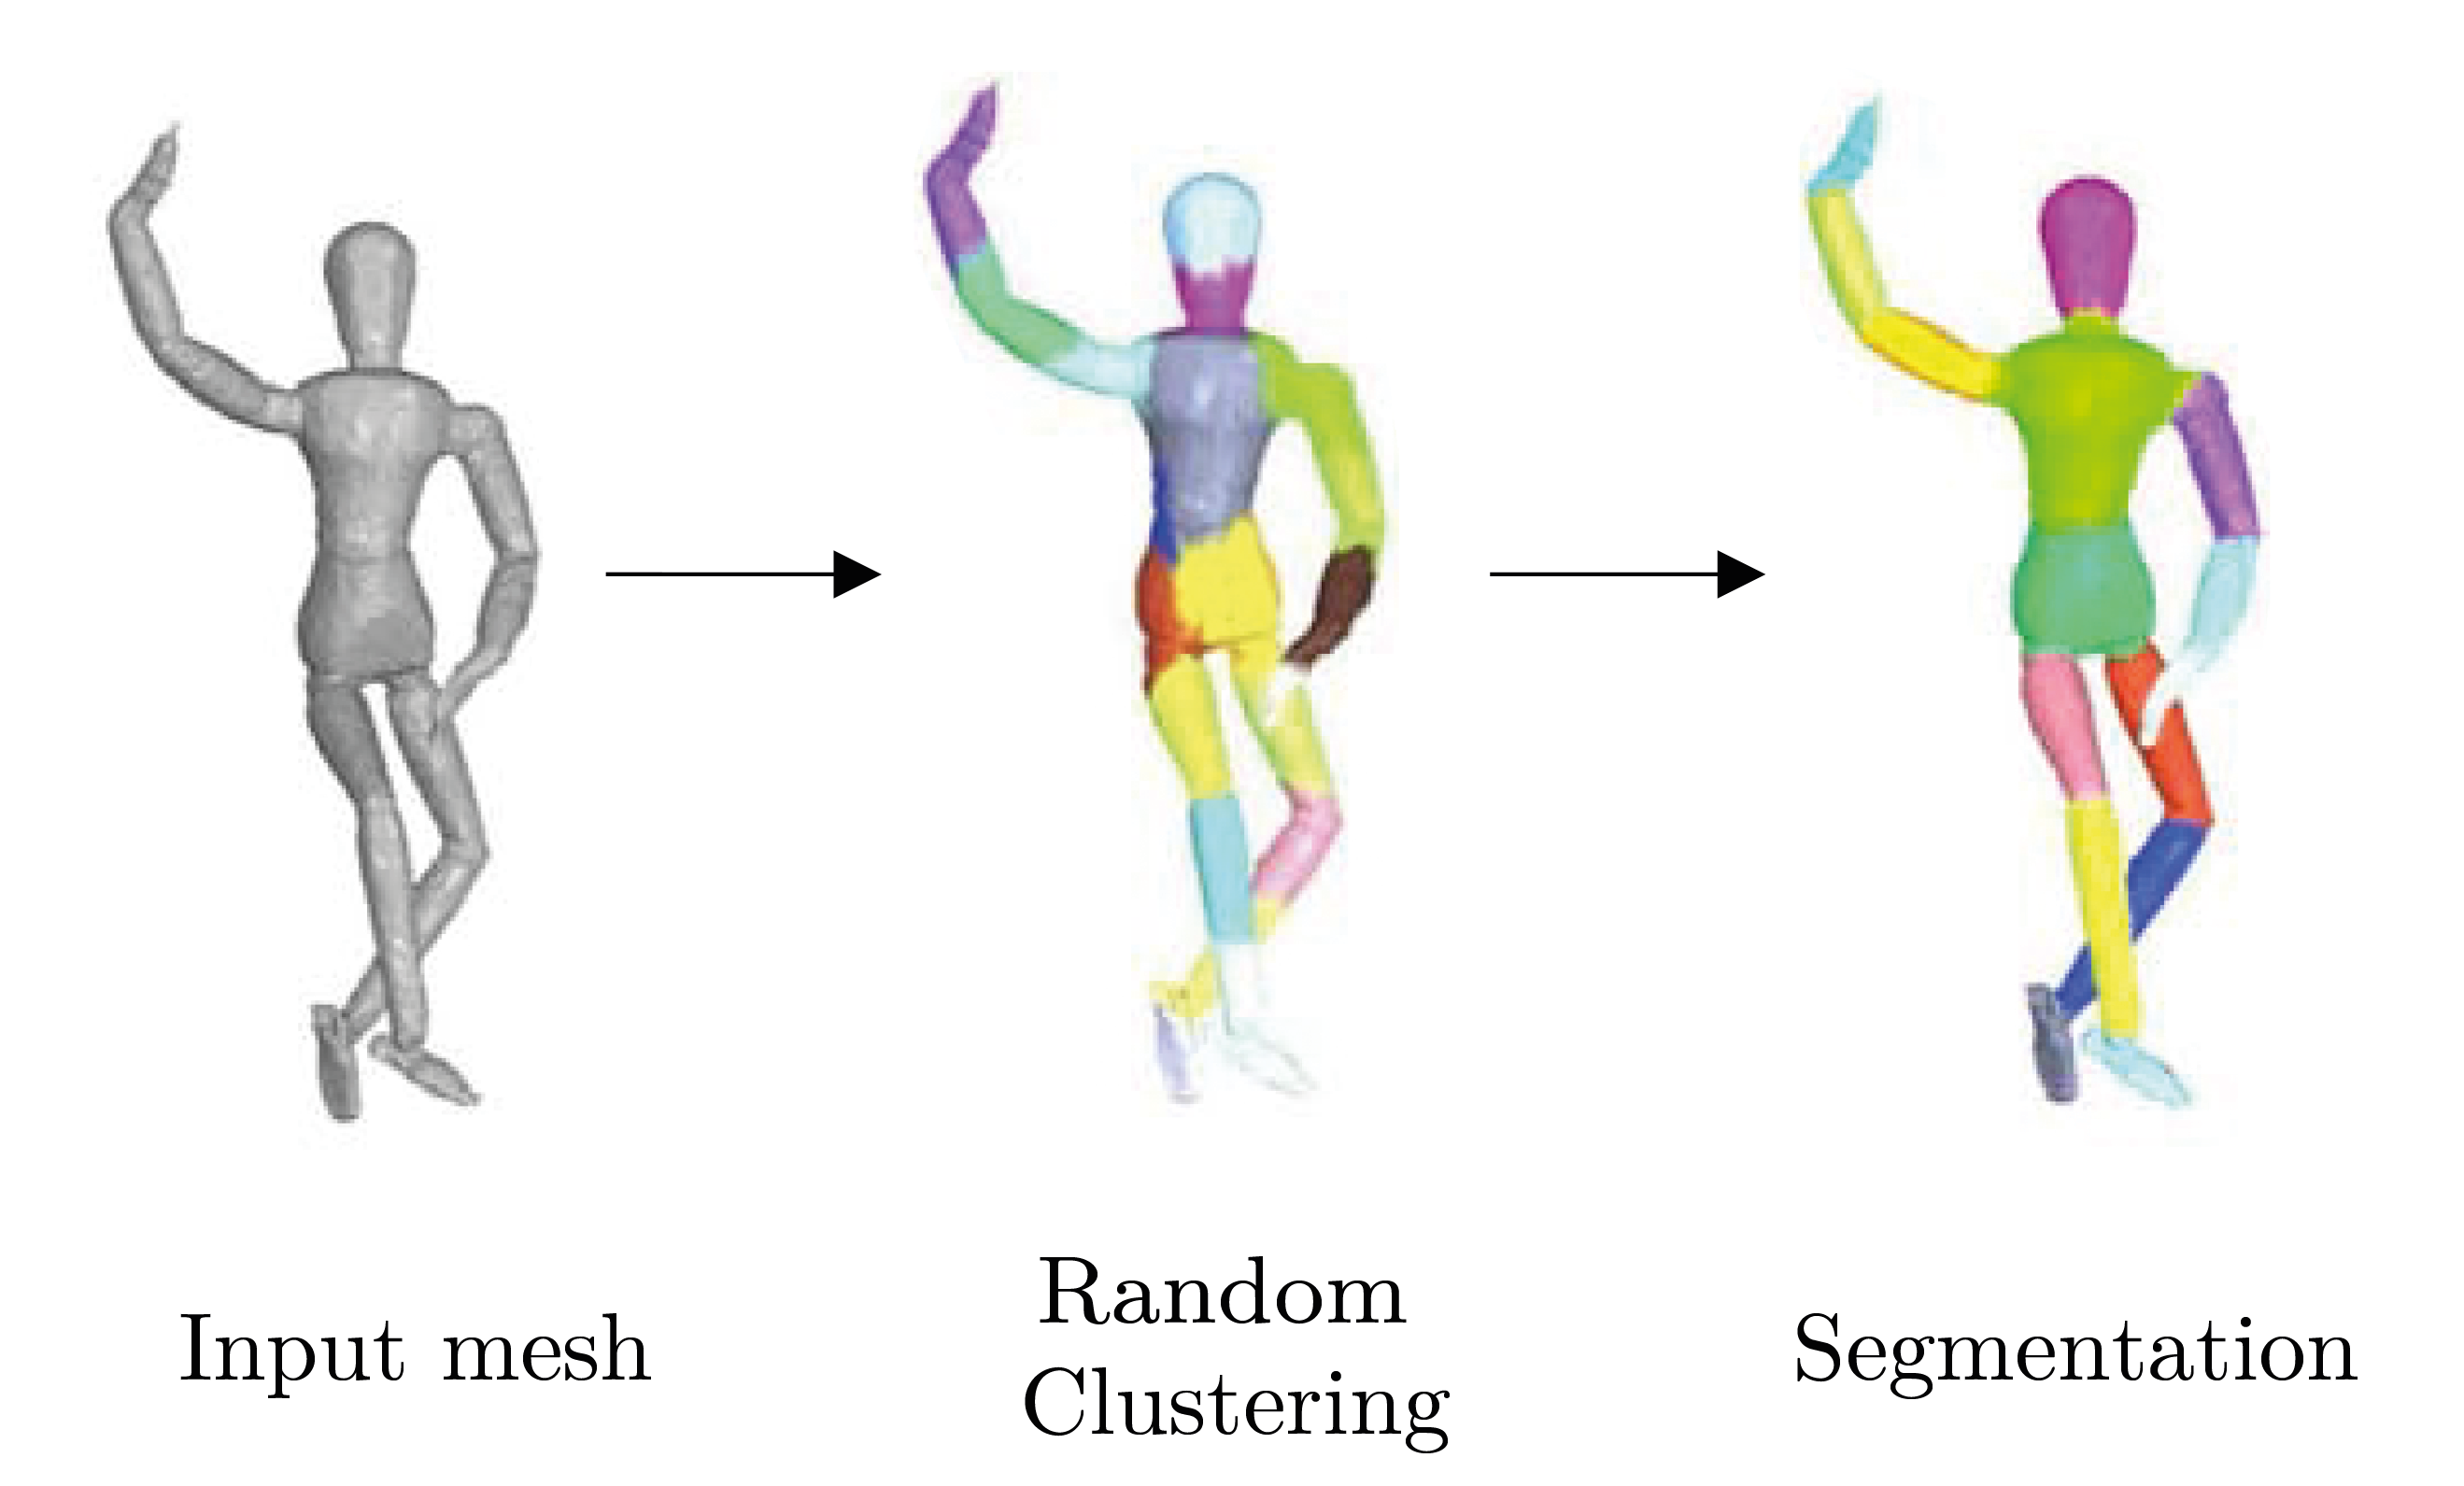
\includegraphics[width=0.7\linewidth]{anguelov}
	\caption{Segmentation a template mesh $M$ into its rigid parts by applying random clustering and a probabilistic framework to iteratively detect associating parts in another mesh \cite{Anguelov04}.}
	\label{fig:correlatedcorrespondance}
\end{figure}
%%
A different approach proposes the recursive detection of body parts by the LRP -- ``largest rigid part'' algorithm \cite {guo2016correspondence}. 
%%
\subsection{LRP}
The LRP algorithm discovers the articulated parts of two objects in different configurations by initially detecting the largest rigid part. This would be the biggest point cluster by applying a single rigid transformation. To reach that, sparse correspondences in combination with RANSAC are implemented. From there, the linking parts are recursively detected by growing clusters from the LRP and reapplying the algorithm. 
%%
\begin{figure}[H]
	\centering\small
	\begin{tabular}{cc}
		\fbox{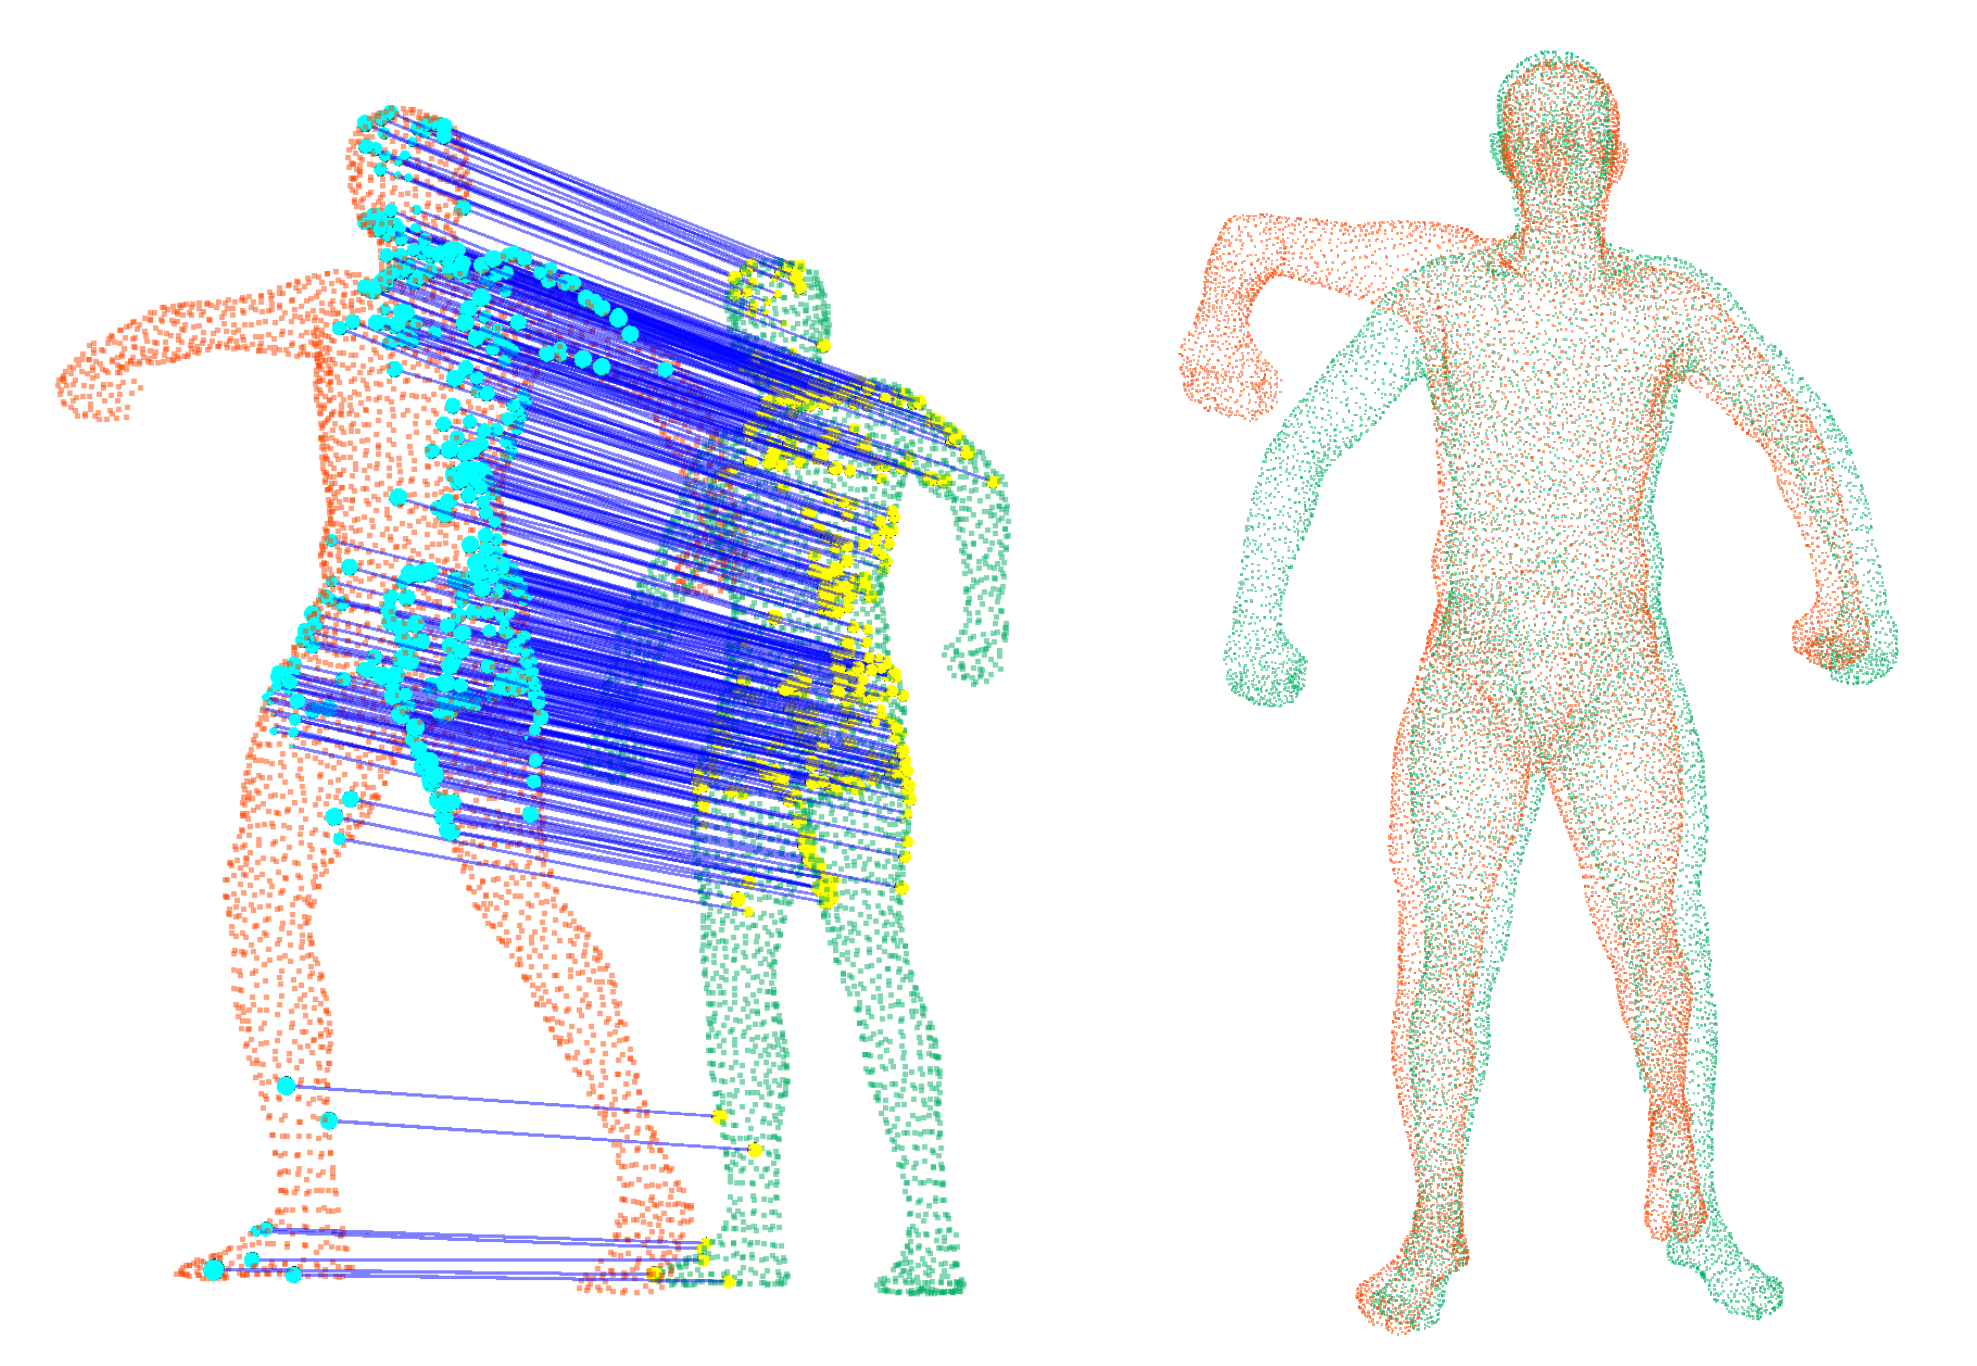
\includegraphics[width=0.45\textwidth]{LRP_body}} &		% JPEG file
		\fbox{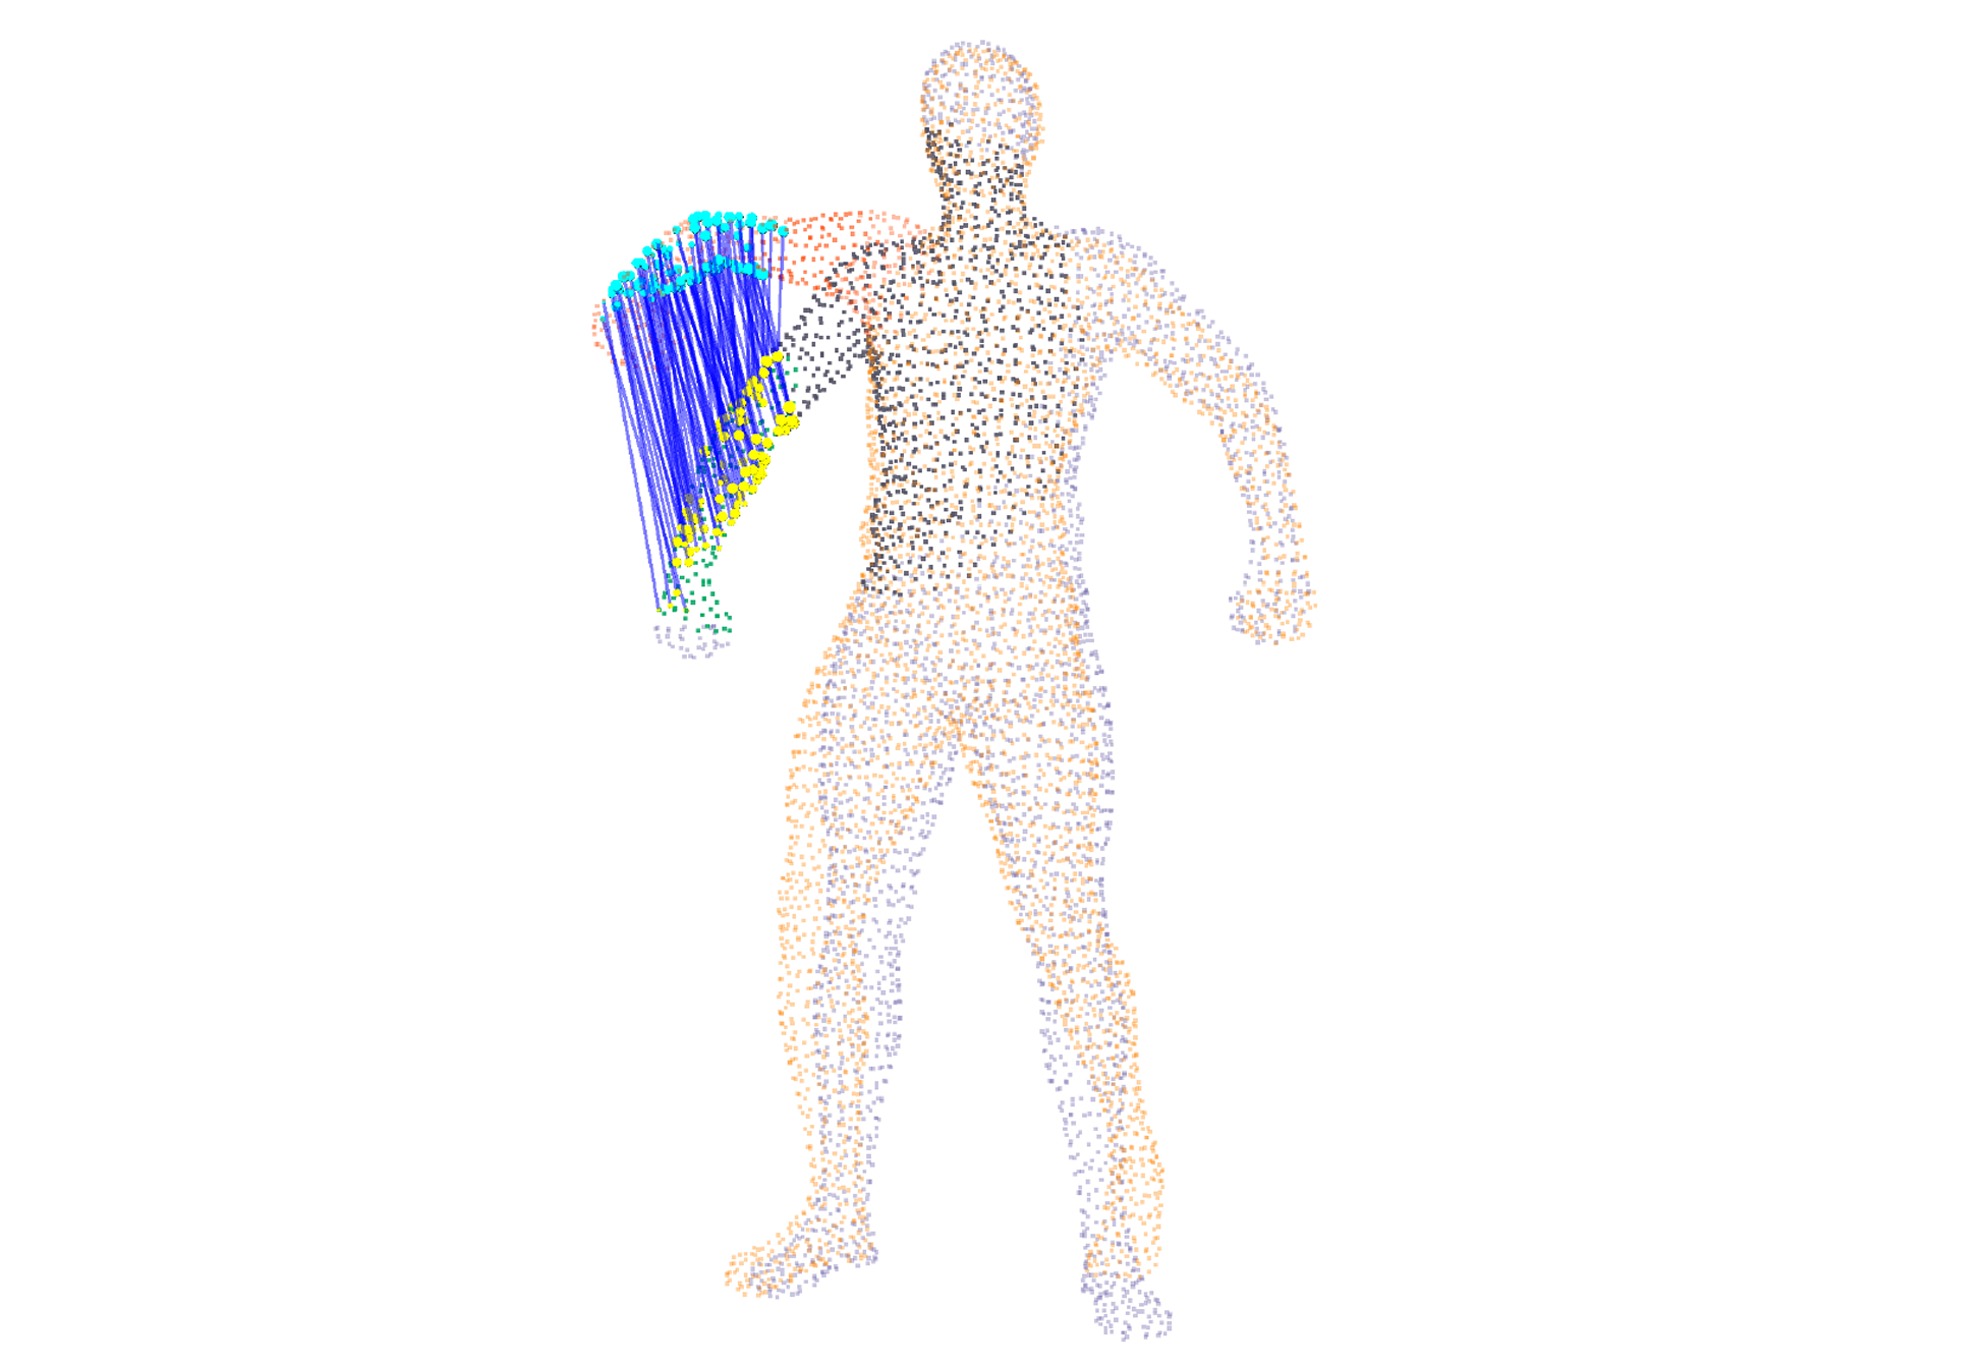
\includegraphics[width=0.45\textwidth]{LRP_arm}} 
		\\	% PNG file
		(a) & (b) 
	\end{tabular}
	\caption{Detecting the largest rigid part of an object~(a), and align the object to recursively detect linking parts to the LRP~(b) \cite{guo2016correspondence}.} 
	\label{fig:LRP_algorithm}
\end{figure}
%%
Another approach is achieved by Symmetrization \cite{Mitra07}, by detecting and aligning the body parts’ symmetry axes of an object(see figure \ref{fig:Symmetrization}). Based on Anguelov \cite{Anguelov04} and Mitra \cite{Mitra07}, Chang et al developed a closely related approach \cite{chang08articulated} \cite{chang09range}.
%%
\begin{figure}[H]
	\centering\small
	\begin{tabular}{cc}
		\fbox{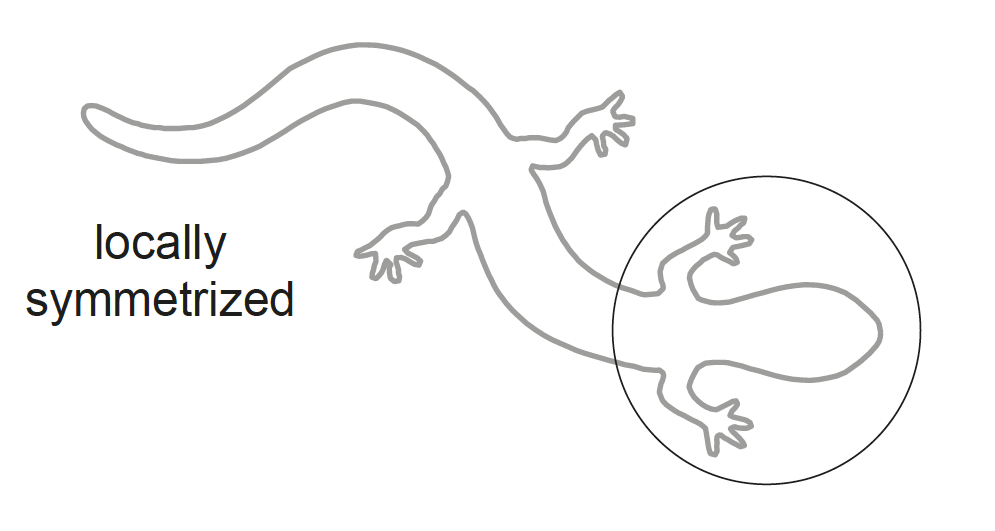
\includegraphics[width=0.45\textwidth]{Symmetrization1}} &		% JPEG file
		\fbox{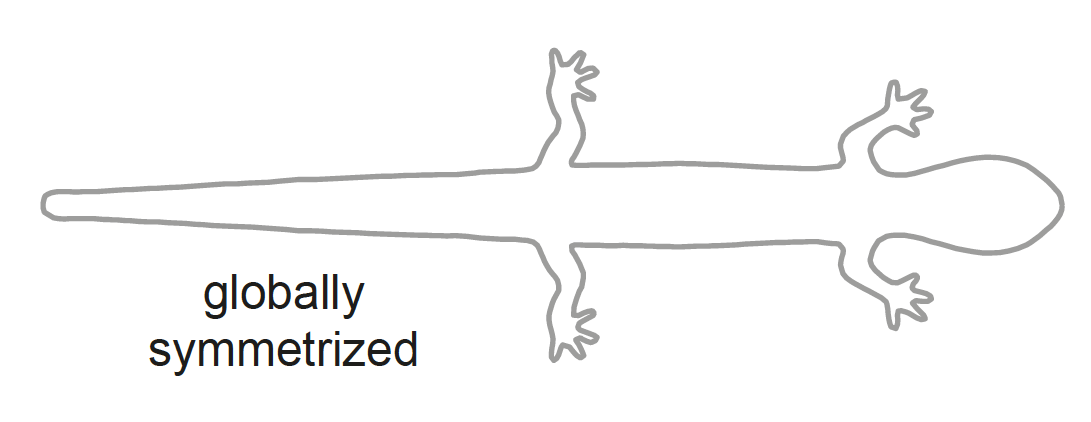
\includegraphics[width=0.45\textwidth]{Symmetrization2}} 
		\\	% PNG file
		(a) & (b) 
	\end{tabular}
	\caption{Detection of the rigid parts of an object by local~(a) and global~(b) Symmetrization \cite{Mitra07}.} 
	\label{fig:Symmetrization}
\end{figure}
%%
\subsection{Possible improvements}
The proposed approaches achieve convincing results concerning the accuracy of the segmentation and the detection of rigid parts. However, they are all computationally expensive and require a considerable number of computation steps to iteratively detect rigid parts in two associated objects. This reflects on the run time of the algorithm which offers therefore great potential for improvements.